\section{The graph matching problem}
\label{sec:ch8:gm}
\paragraph*{Co-authored with Ali Saad-Eldin}
At this point, we've spent a good deal of time deciding how to determine whether or not two networks are distinct in some way. We first saw this example (in the general case) when the networks were samples of $RDPG_n(X)$ random networks, wherein we could use the latent position and latent distribution test to see whether the underlying random networks were different. Next, we saw how in the special case that the networks were samples of $SBM_n(\vec z, B)$ random networks, we could use Fisher's exact tests and modified versions of chi-squared tests to investigate whether the block matrices differed.

% In this section, we'll turn this around with the \textit{graph matching problem}. The \textit{graph matching problem} is the problem of uncovering similarities between a pair of networks. Let's take a look at a running example in Case Study \ref{box:ch8:gm:ex}.

In this section, we'll turn this around with the \textit{graph matching problem}. The \textit{graph matching problem} is the problem of finding a good match between the indices of the nodes of two networks.

\begin{floatingbox}[h]\caption{Case Study: Graph matching across social networks}
\label{box:ch8:gm:ex}
You work at Facebook and Twitter, but there’s been a terrible incident on the Twitter end. All Twitter users’ names and handles have been somehow been deleted! Your bosses have tasked you with recovering the lost information. How might you go about doing this? Luckily, you have a great resource at your disposal: the Facebook social network. You know all Facebook users and who they are friends with, and since you’ve only lost the Twitter usernames, you can still figure out which unnamed Twitter users follow each other. You decide to use the Facebook network connectivity data to re-label the Twitter social network. Alternatively, you can say the we are ``aligning’’ or ``matching'' Twitter to Facebook. \\

In the two social networks above, each user is a node and an edge exists if two users are friends. We'll define the Facebook and Twitter networks as $F$ and $T$ respectively, with associated adjacency matrices $A^{(F)}$ and $A^{(T)}$. Aligning the nodes of two networks is known as graph matching, because we are matching the node indices of one network (or, graph) to another. This can also be thought of as a mapping; that is, based on the neighbors of a node in $F$, you find a node in $T$ with the most similar neighborhood structure, then give the two nodes the same index. In other words, one of our Twitter users will be assigned the user name of the Facebook user with the most connections in common. This is done for the whole network, with the end result being that overall the structure is best preserved.
\end{floatingbox}

\subsection{Brute Forcing is Infeasible}
If you were to pick randomly, there would be an infeasibly large number of ways to match the nodes of two networks. In fact, for network pairs with $n$ nodes, there are $n!$ (factorial) possible mappings. For example, when $n=100$, there are more than $10^{157}$ possible matchings. So, our task is to figure out which mapping is best without the computationally gargantuan task of checking each one. For a thorough review of the history of different ways of approaching this problem, see \cite{Livi2013Aug}.

\subsection{Defining a similarity metric}

First, we need a metric. We want this metric to be small when two networks, $f\left(A^{(1)}, A^{(2)}\right)$, are similar, and large when they are not. For graph matching, we use the Frobenius distance from Concept \ref{box:ch7:twosample:frobnorm}:
\begin{align*}
    f\left(A^{(1)}, A^{(2)}\right) &= \left\|A^{(1)} - A^{(2)}\right\|_F.
\end{align*}

To understand this functionally, consider the best possible case where where the two networks are identical: $A=B$. 

\begin{align*}
A^{(1)} = 
\begin{array}{cc} &
\begin{array}{ccc} 0 & 1 & 2 \end{array}
\\
\begin{array}{cc}
0 \\
1 \\
2 \end{array}
&
\left[
\begin{array}{ccc}
0 & 1 & 1\\
1 & 0 & 1\\
1 & 1 & 0\end{array}
\right]\end{array}
\quad \quad
A^{(2)} = 
\begin{array}{cc} &
\begin{array}{ccc} 0 & 1 & 2 \end{array}
\\
\begin{array}{ccc}
0 \\
1 \\
2 \end{array}
&
\left[
\begin{array}{ccc}
0 & 1 & 1\\
1 & 0 & 1\\
1 & 1 & 0\end{array}
\right]\end{array}
\\
A^{(1)}-A^{(2)} =
\begin{array}{cc} &
\begin{array}{ccc} 0 & 1 & 2 \end{array}
\\
\begin{array}{ccc}
0 \\
1 \\
2 \end{array}
&
\left[
\begin{array}{ccc}
0 & 0 & 0\\
0 & 0 & 0\\
0 & 0 & 0\end{array}
\right]\end{array}
\\
\left\|A^{(1)} - A^{(2)}\right\|_F^2 = 0.
\end{align*}
As we see above, the difference will be a matrix of all zeros, and taking the squared Frobenius norm will then yield $f\left(A^{(1)}, A^{(2)}\right) = 0$. This is because all of the element-wise differences $a_{ij}^{(1)} - a_{ij}^{(2)}$ are just zero, and hence both their square (and sum) will also be zero. Below we remove one edge from $A^{(2)}$:

\begin{align*}
A^{(1)} = 
\begin{array}{cc} &
\begin{array}{ccc} 0 & 1 & 2 \end{array}
\\
\begin{array}{ccc}
0 \\
1 \\
2 \end{array}
&
\left[
\begin{array}{ccc}
0 & 1 & 1\\
1 & 0 & 1\\
1 & 1 & 0\end{array}
\right]\end{array}
\quad \quad
A^{(2)} = 
\begin{array}{cc} &
\begin{array}{ccc} 0 & 1 & 2 \end{array}
\\
\begin{array}{ccc}
0 \\
1 \\
2 \end{array}
&
\left[
\begin{array}{ccc}
0 & 1 & 1\\
1 & 0 & 0\\
1 & 0 & 0\end{array}
\right]\end{array}
\\
A^{(1)} - A^{(2)} =
\begin{array}{cc} &
\begin{array}{ccc} 0 & 1 & 2 \end{array}
\\
\begin{array}{ccc}
0 \\
1 \\
2 \end{array}
&
\left[
\begin{array}{ccc}
0 & 0 & 0\\
0 & 0 & 1\\
0 & 1 & 0\end{array}
\right]\end{array}
\\
\left\|A^{(1)} - A^{(2)}\right\|_F^2 = 2.
\end{align*}

Because these networks are unweighted and undirected, we are effectively counting the total number of disagreements in the adjacency matrices between $A^{(1)}$ and $A^{(2)}$.

\subsubsection*{Graph Matching Small Networks}


Instead of (1) and (2), let's use $T$ and $F$ for Twitter and Facebook. our two networks, $A^{(T)}$ and $A^{(F)}$, have four nodes each: $\{1, 2, 3, 4\}$ for $A^{(T)}$, and $\{a, b, c, d\}$ for $A^{(F)}$. In this case, the nodes represent people within the social networks, and the edges represent whether two people are connected on the social networking site. In this case, we will assume we have a node correspondence:
\begin{enumerate}
    \item Person $0$ on Twitter is person $a$ on Facebook,
    \item Person $1$ on Twitter is person $b$ on Facebook,
    \item Person $2$ on Twitter is person $c$ on Facebook,
    \item Person $3$ on Twitter is person $d$ on Facebook.
\end{enumerate}

\paragraph*{Node order is irrelevant if node correspondence is respected}

The corresponding adjacency matrices of the two networks are equal to each other when the nodes are laid out for $A^{(T)}$ as $\{0, 1, 2, 3\}$, and when the nodes are laid out for $A^{(F)}$ as $\{a,b,c,d\}$. The two networks are illustrated, with their nodes laid out with respect to the node correspondence, in Figure \ref{fig:ch8:gm:ex}(A).

\begin{align*}
A^{(F)} = 
\begin{array}{cc} &
\begin{array}{cccc} 0 & 1 & 2 & 3 \end{array}
\\
\begin{array}{cccc}
0 \\
1 \\
2 \\
3 \end{array}
&
\left(
\begin{array}{cccc}
0 & 1 & 1 & 0\\
1 & 0 & 0 & 1\\
1 & 0 & 0 & 1\\
0 & 1 & 1 & 0\end{array}
\right)\end{array}
\quad \quad
A^{(T)} = 
\begin{array}{cc} &
\begin{array}{cccc} a & b & c & d \end{array}
\\
\begin{array}{ccc}
a \\
b \\
c \\
d \end{array}
&
\left(
\begin{array}{cccc}
0 & 1 & 1 & 0\\
1 & 0 & 0 & 1\\
1 & 0 & 0 & 1\\
0 & 1 & 1 & 0\end{array}
\right)\end{array} \\
\left|A^{(F)} - A^{(T)}\right| = \left[
\begin{array}{cccc}
0 & 0 & 0 & 0\\
0 & 0 & 0 & 0\\
0 & 0 & 0 & 0\\
0 & 0 & 0 & 0\end{array}
\right]
\end{align*}

\begin{figure}[h]
    \centering
    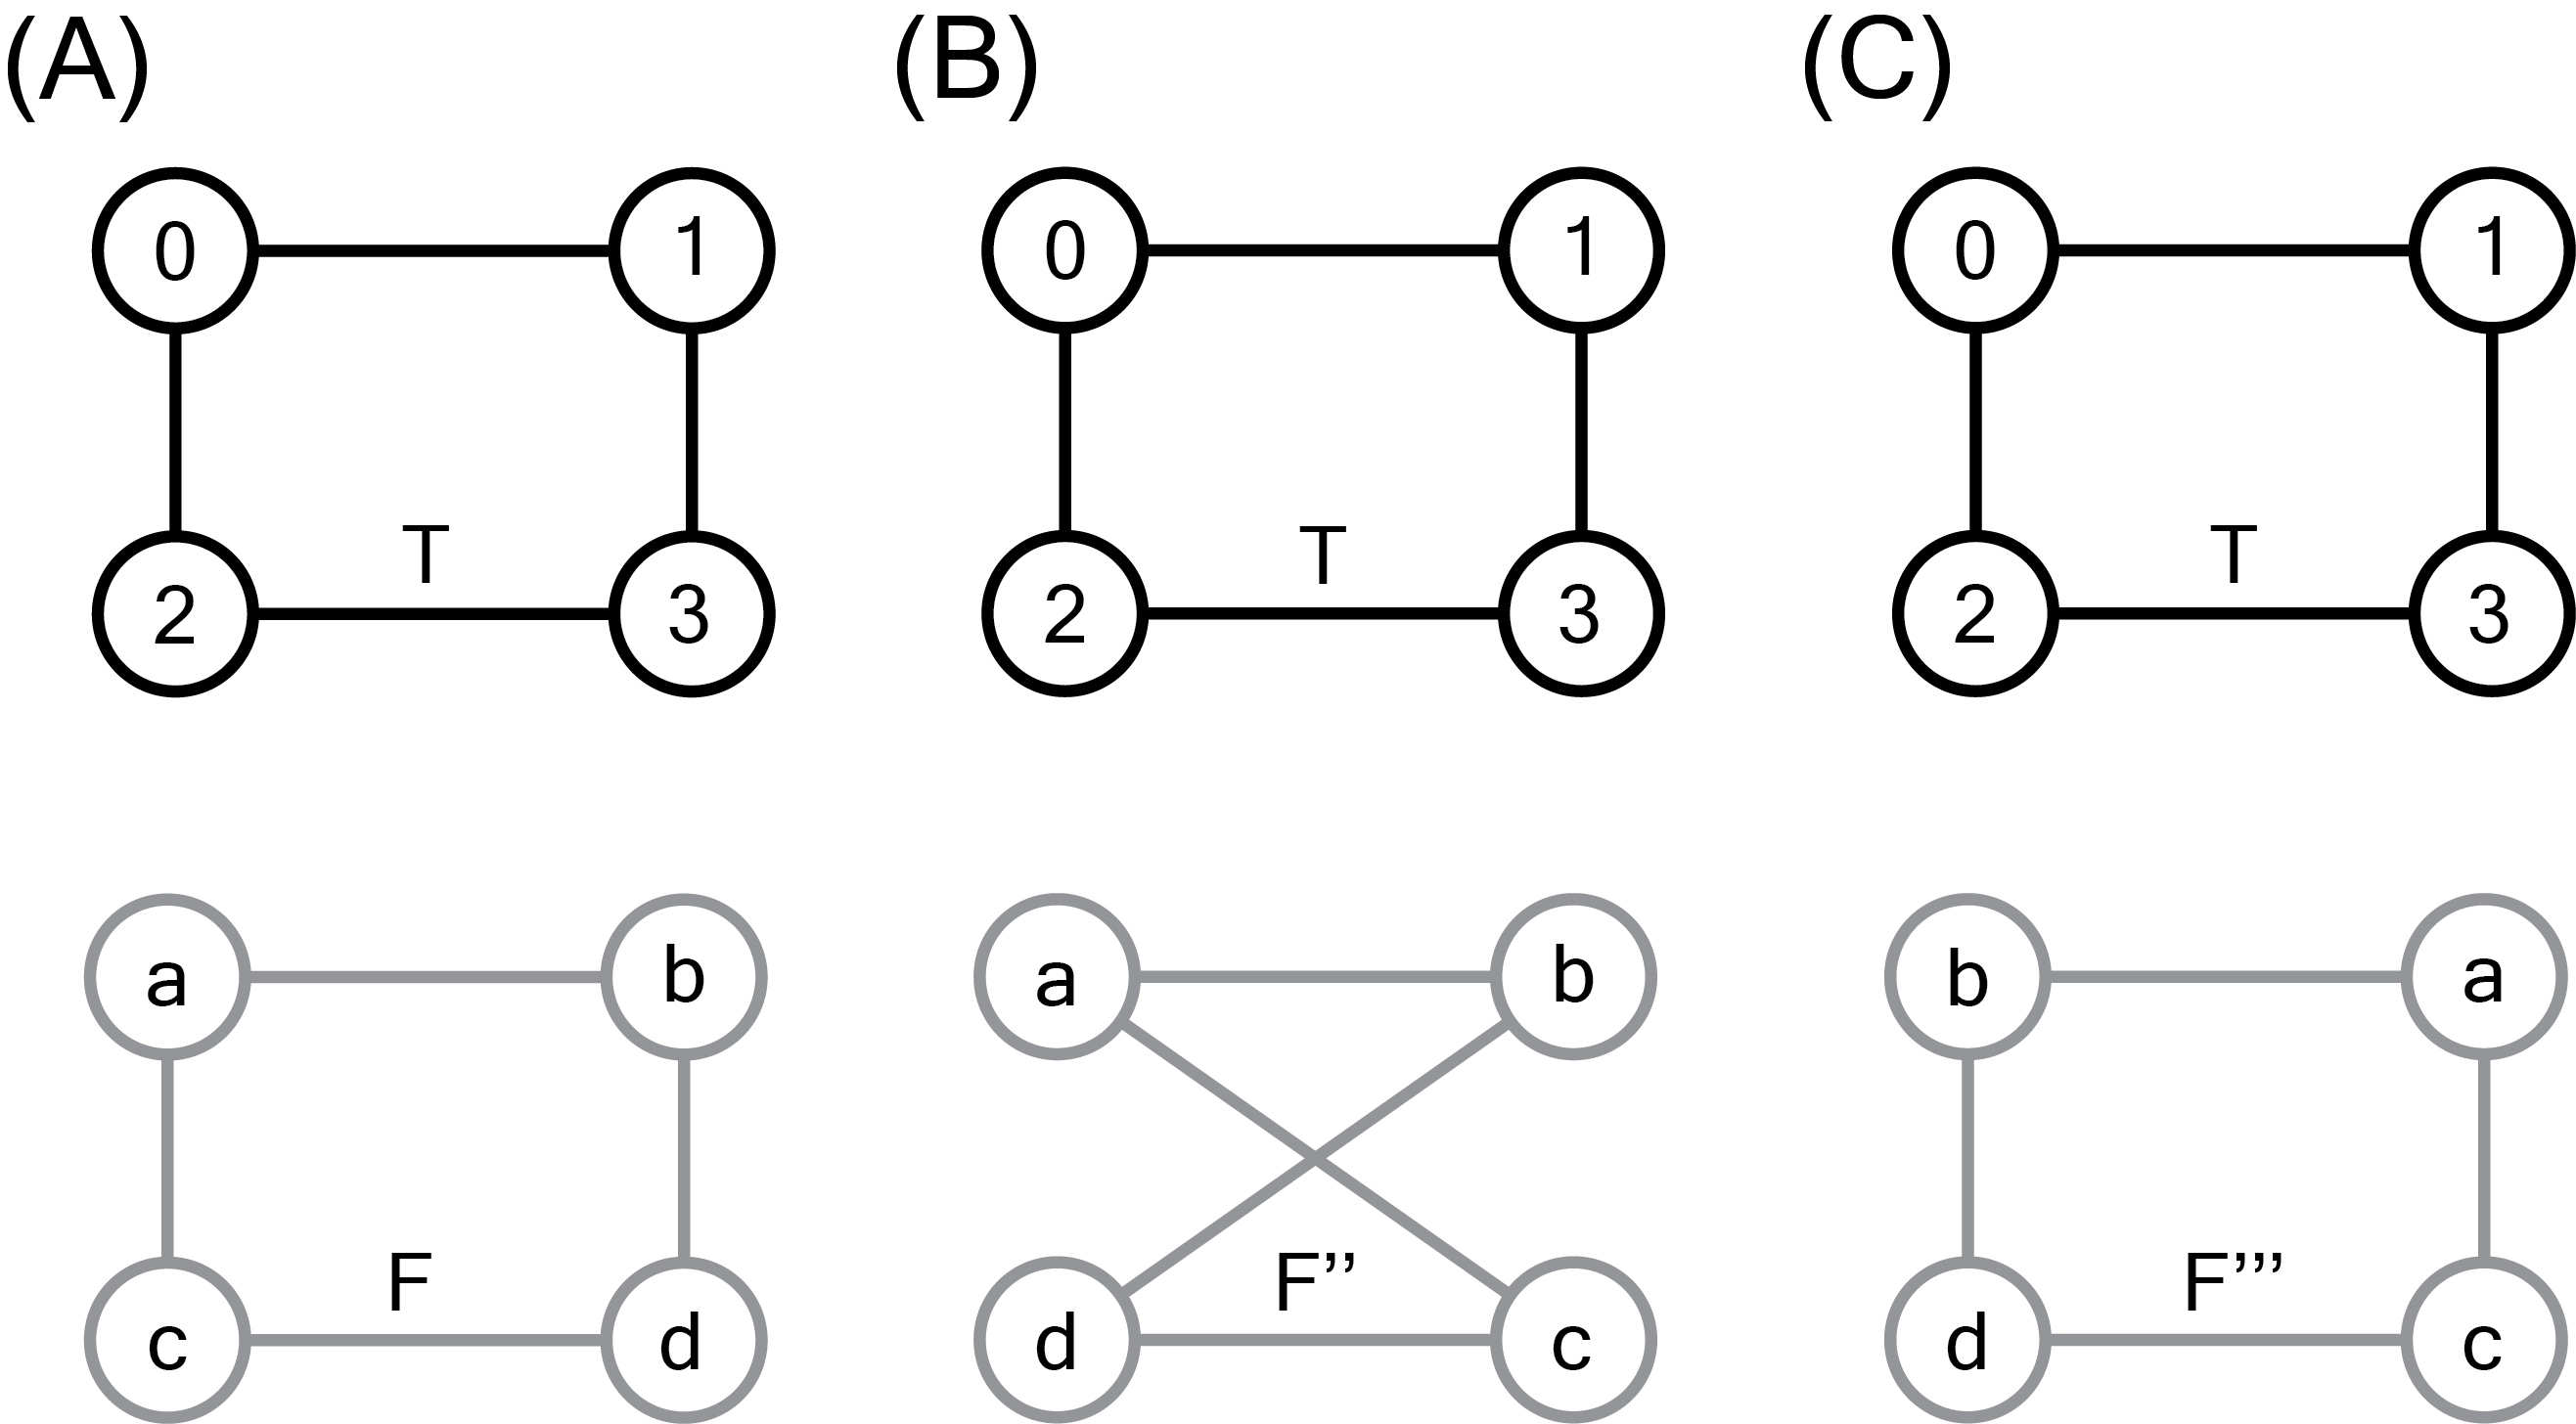
\includegraphics[width=\linewidth]{applications/ch8/Images/gm_ex.png}
    \caption[Social network $4$ node graph matching example]{\textbf{(A)} the social networks, with the nodes aligned. \textbf{(B)} the social networks, with the nodes mis-aligned. \textbf{(C)} the social networks, with the nodes mis-aligned, but with the topology of the network identical.}
    \label{fig:ch8:gm:ex}
\end{figure}
    
We can see above that $f(A_T, A_B) = 0$. By ordering the nodes, we're claiming that there is some kind of match between the Twitter and Facebook nodes. Ordering the adjacency matrices under this claim will give us a low edge disagreement (here, just zero). 

If we permute the node indices of both networks in the same way, we can still find a low edge disagreement. Let's reorder the nodes for Twitter and Facebook as $\{2, 0, 1, 3\}$ and $\{c, a, b, d\}$ respectively. We will call these new adjacency matrices $A_T'$ and $A_F'$ respectively:

\begin{align*}
A^{(T)}' = 
\begin{array}{cc} &
\begin{array}{cccc} 2 & 0 & 1 & 3 \end{array}
\\
\begin{array}{cccc}
2 \\
0 \\
1 \\
3 \end{array}
&
\left[
\begin{array}{cccc}
0 & 1 & 0 & 1 \\
1 & 0 & 1 & 0\\
0 & 1 & 0 & 1\\
1 & 0 & 1 & 0
\end{array}
\right]\end{array}
\quad \quad
A^{(F)}' = 
\begin{array}{cc} &
\begin{array}{cccc} c & a & b & d \end{array}
\\
\begin{array}{ccc}
c \\
a \\
b \\
d \end{array}
&
\left[
\begin{array}{cccc}
0 & 1 & 0 & 1 \\
1 & 0 & 1 & 0\\
0 & 1 & 0 & 1\\
1 & 0 & 1 & 0
\end{array}
\right]\end{array} \\
\left|A^{(T)}' - A^{(F)}'\right| = \left[
\begin{array}{cccc}
0 & 0 & 0 & 0\\
0 & 0 & 0 & 0\\
0 & 0 & 0 & 0\\
0 & 0 & 0 & 0\end{array}
\right]
\end{align*}

Even though the ordering of the nodes is different, like goes with like: the first node for Twitter is node $2$ and the first node for Facebook is node $c$, the second node for Twitter is $0$ and the second node for Facebook is node $a$, so on and so forth. The node orderings preserve the correspondence between the nodes of Twitter with the nodes of Facebook.

\paragraph*{Networks rarely come pre-ordered}

The ordering of a network's nodes in an adjacency is arbitrary, which can often make it hard to tell whether two networks are the same. 

Let's say we had an arbitrary ordering of the nodes for Facebook, which was a little bit different from the one which we just saw: The nodes are ordered $\{a, b, d, c\}$ instead of $\{a, b, c, d\}$. Twitter's nodes are still ordered as $\{0, 1, 2, 3\}$. This is illustrated in Figure \ref{fig:ch8:gm:ex}(B). We use $A^{(F)``}$ to denote the new ordering. The adjacency matrices are no longer equal:

\begin{align*}
A^{(T)} = 
\begin{array}{cc} &
\begin{array}{cccc} 0 & 1 & 2 & 3 \end{array}
\\
\begin{array}{cccc}
0 \\
1 \\
2 \\
3 \end{array}
&
\left[
\begin{array}{cccc}
0 & 1 & 1 & 0\\
1 & 0 & 0 & 1\\
1 & 0 & 0 & 1\\
0 & 1 & 1 & 0\end{array}
\right]\end{array}
\quad \quad
A^{(F)}'' = 
\begin{array}{cc} &
\begin{array}{cccc} a & b & d & c \end{array}
\\
\begin{array}{cccc}
a \\
b \\
d \\
c \end{array}
&
\left(
\begin{array}{cccc}
0 & 1 & 0 & 1\\
1 & 0 & 1 & 0\\
0 & 1 & 0 & 1\\
1 & 0 & 1 & 0\end{array}
\right)\end{array} \numberthis \label{eqn:ch8:gm:fb_perm:e1}\\
\left|A^{(T)} - A^{(F)}''\right| = \left[
\begin{array}{cccc}
0 & 0 & 1 & 1\\
0 & 0 & 1 & 1\\
1 & 1 & 0 & 0\\
1 & 1 & 0 & 0\end{array}
\right]
\end{align*}
    
Our similarity metric changes as well: $f\left(A^{(T)}, A^{(F)}''\right) = 8$, since there are $8$ entries which are different in the adjacency matrices between $A^{(T)}$ and $A^{(F)}''$. This might seem a bit high, but remember - the network is undirected, so adjacency disagreements are effectively counted twice (a single edge disagreement for an edge $(i,j)$ also yields a disagreement for edge $(j, i)$, since the adjacency matrix is symmetric). By comparing the nodes of Twitter and Facebook with the nodes misaligned, we have effectively broken the node correspondence between the nodes of Twitter and Facebook. 

Let's explore how to manipulate our adjacency matrices such that we can find alignments that match well.

\begin{floatingbox}[h]\caption{Low numbers of edge disagreements do not imply node correspondence}

Let's imagine that we mix the ordering of the nodes for Facebook a third time, instead using $\{b, a, d, c\}$, to yield another adjacency matrix $A^{(F)}'''$, illustrated in Figure \ref{fig:ch8:gm:ex}(C). Note that the adjacency matrices are identical for $A^{(F)}'''$ and $A^{(T)}$, despite the face that the nodes for Facebook are not ordered with respect to the node correspondence of the Twitter network:

\begin{align*}
A^{(T)} = 
\begin{array}{cc} &
\begin{array}{cccc} 0 & 1 & 2 & 3 \end{array}
\\
\begin{array}{cccc}
0 \\
1 \\
2 \\
3 \end{array}
&
\left[
\begin{array}{cccc}
0 & 1 & 1 & 0\\
1 & 0 & 0 & 1\\
1 & 0 & 0 & 1\\
0 & 1 & 1 & 0\end{array}
\right]\end{array}
\quad \quad
A^{(F)}''' = 
\begin{array}{cc} &
\begin{array}{cccc} b & a & d & c \end{array}
\\
\begin{array}{ccc}
b \\
a \\
d \\
c \end{array}
&
\left[
\begin{array}{cccc}
0 & 1 & 1 & 0\\
1 & 0 & 0 & 1\\
1 & 0 & 0 & 1\\
0 & 1 & 1 & 0\end{array}
\right]\end{array} \\
\left|A^{(T)} - A^{(F)}'''\right| = \left[
\begin{array}{cccc}
0 & 0 & 0 & 0\\
0 & 0 & 0 & 0\\
0 & 0 & 0 & 0\\
0 & 0 & 0 & 0\end{array}
\right]
\end{align*}

This illustrates that the adjacency matrices can be identical even when we do not have a correspondence of the nodes between the two networks, which presents a challenge and limitation for the graph matching problem that you should be aware of. Formally, this means that if two networks are identical (up to an ordering of the nodes), there may be multiple ways to orient the nodes of the networks in which you obtain no edge disagreements. Stated another way, we could have multiple different networks where the topology (as indicated by the adjacency matrix) is the same.
\end{floatingbox}
\subsection{Permutation Matrices}

Permutation matrices are commonly used as a method to move around the rows and columns of a square matrix. A \textit{permutation matrix} is a matrix where, for every row and column, exactly one entry has a value of one. 
\subsubsection*{$P^\top A$ moves the rows}

Let's consider a matrix $A$ where all entries of the first row have a value of one, all entries of the second row have a value of two, all entries of the third row have a value of three, and all entries of the fourth row have a value of four. This matrix is shown in Figure \ref{fig:ch8:gm:perm}(A.I). We can apply a permutation matrix $P$ to swap the rows around with the following heuristic: If the matrix $P$ has an entry $p_{ji}$ which is one, then in the resulting matrix, the row $i$ will be the row $j$ from the matrix we permuted. 

For instance, in Figure \ref{fig:ch8:gm:perm}(A.II), the values $p_{12}$, $p_{23}$, $p_{34}$, and $p_{41}$ all have values of one, which means we will reorder the rows of $A$ so that $P^\top A$ will have the top row being the second row from the original matrix (and will have a value of two), the second row will be the third row from the original matrix (and will have a value of three), the third row will be the fourth row from the original matrix (and will have a value of four), and the fourth row will be the first row from the original matrix (and will have a value of one. 

We apply this ``row'' permutation with the matrix multiplication $P^\top A$:

\begin{lstlisting}[style=python]
import numpy as np

A = np.array([
    [1,1,1,1],
    [2,2,2,2],
    [3,3,3,3],
    [4,4,4,4]
])

P = np.array([
    [0,0,0,1],
    [1,0,0,0],
    [0,1,0,0],
    [0,0,1,0]
])

row_reordering = P.T @ A
\end{lstlisting}

We show a plot of the resulting row permutation in Figure \ref{fig:ch8:gm:perm}(A.III). Note that the row with a value of $1$ has been ``shifted'' to row $4$, and the values of rows $1$ through $3$ are $2$ through $4$ respectively. This is because of the way the rows/columns of the permutation matrix were arranged, as-per above.

\begin{figure}
    \centering
    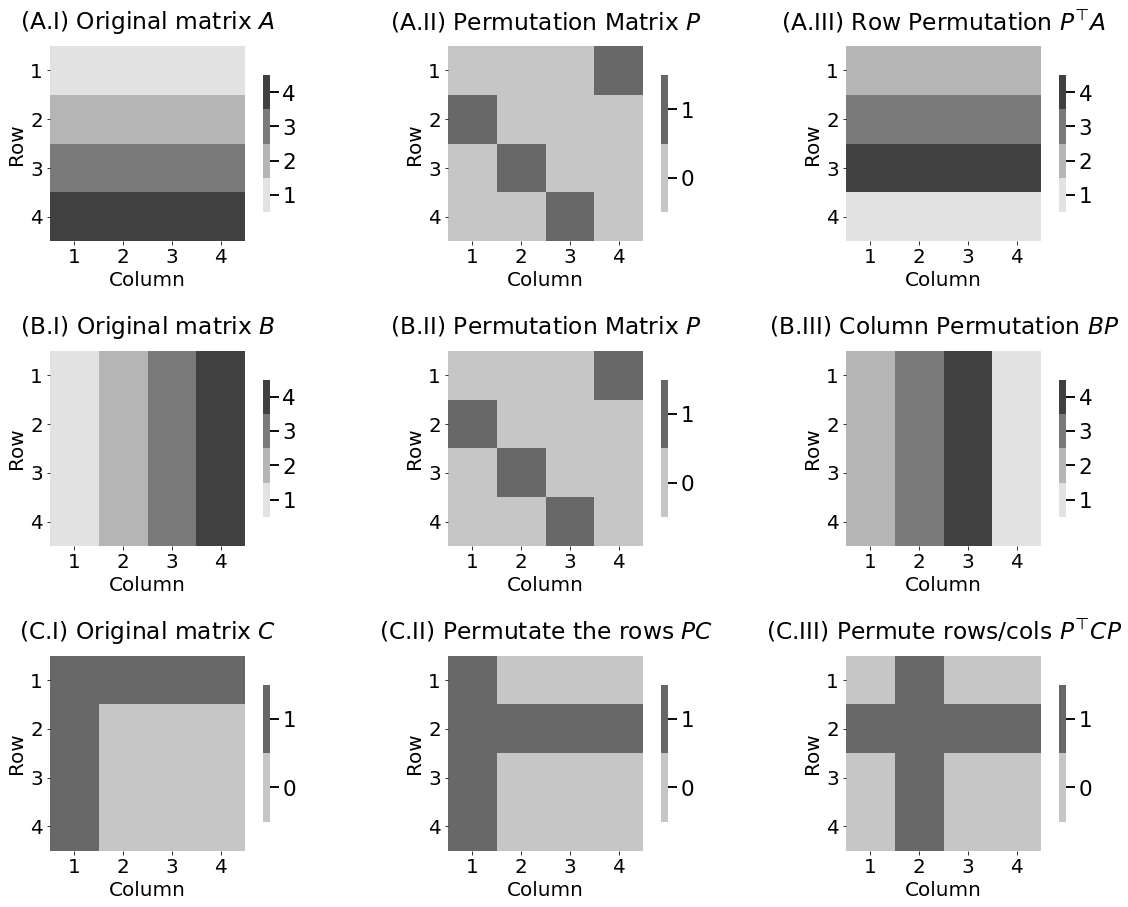
\includegraphics[width=\linewidth]{applications/ch8/Images/gm_perm.png}
    \caption[Permutation matrices]{Row \textbf{(A)} shows a row permutation via pre-multiplication by $P^\top$, Row \textbf{(B)} shows a column permutation via post-multiplication by $P$, and row \textbf{(C)} shows a row and column permutation via pre-multiplication by $P^\top$ and post multiplication by $P$.}
    \label{fig:ch8:gm:perm}
\end{figure}
\subsubsection*{$BP$ moves the columns}

Likewise, a column permutation behaves very similarly. Let's now consider a matrix $B$, where the first column has a value of one, the second column has a value of two, the third column has a value of three, and the fourth column has a value of four, shown in Figure \ref{fig:ch8:gm:perm}(B.I). We use the same permutation matrix, where here, $p_{ji}$ indicates that column $i$ of the new matrix will be column $j$ from the matrix before the permutation was applied. This permutation is shown again in Figure \ref{fig:ch8:gm:perm}(B.II). We apply the column permutation matrix as $BP$:

\begin{lstlisting}[style=python]
B = np.array([
    [1,2,3,4],
    [1,2,3,4],
    [1,2,3,4],
    [1,2,3,4]
])

P = np.array([
    [0,0,0,1],
    [1,0,0,0],
    [0,1,0,0],
    [0,0,1,0]
])

column_reordering = B @ P
\end{lstlisting}

We show a plot of the resulting column permutation in Figure \ref{fig:ch8:gm:perm}(B.III). Note that the column with a value of $1$ has been ``shifted'' to column $4$, and the values of columns $1$ through $3$ are now $2$ through $4$ respectively. 

\subsubsection*{$P^\top DP$ moves the rows and columns concurrently}

As an interesting property of permutation matrices, we can apply these operations sequentially to reorder both the rows and columns of a matrix. Consider, for instance, a permutation matrix where row/column $1$ of the original matrix becomes row/column $2$ of the new matrix, and likewise, row/column $2$ of the original matrix becomes row/column $1$ of the new matrix. We'll consider a matrix $C$ where the first row and first column both have entries of all ones, and the rest of the matrix has the value zero. This matrix $C$ is shown in Figure \ref{fig:ch8:gm:perm}(C.I):

\begin{lstlisting}[style=python]
C = np.array([
    [1,1,1,1],
    [1,0,0,0],
    [1,0,0,0],
    [1,0,0,0]
])

P = np.array([
    [0,1,0,0],
    [1,0,0,0],
    [0,0,1,0],
    [0,0,0,1]
])

row_reordering = P.T @ C
row_column_reordering = row_reordering @ P
\end{lstlisting}

When we pre-multiply by $P^\top$, we end up ``swapping'' row $1$ with row $2$, as we would expect from what we learned in Figure \ref{fig:ch8:gm:perm}(A). When we post-multiply $P^\top C$ by $P$, we end up ``swapping'' columns $1$ and $2$, as we would expect from what we learned in Figure \ref{fig:ch8:gm:perm}(B). This results in jointly swapping the rows and columns $1$ and $2$, shown in Figure \ref{fig:ch8:gm:perm}(C.III). If $C$ were an adjacency matrix with nodes indexed $\{1, 2, 3, 4\}$, this would have the effect of permuting the node ordering of the adjacency matrix to $\{2, 1, 3, 4\}$.

\subsubsection*{Using concurrent row and column permutations on adjacency matrices}

For our networks, remember that the adjacency matrix is the matrix $A$ where the entry $a_{ij}$ represents whether or not there is an edge between nodes $i$ and $j$. The key aspect is that the indexing for the adjacency matrix, $ij$, is an indexing over a single set: the nodes. This means that if we want to reorder the adjacency matrix by moving around the nodes, we need to move both the rows and the columns concurrently, since the node ordering is what is being permuted. If we had a permutation of the nodes given by $P$, we would correspondingly reorder the adjacency matrix by permuting the rows and columns of $A$ by using $P^\top AP$.


\paragraph*{Permutation Matrices are unshuffled by their transpose}

Let's suppose that we have a permutation matrix, $P$. We remember from above that a permutation matrix is a matrix where every row and every column has a single entry which takes a value of one. Let's assume that $p_{ji} = 1$, which means that if we were to use the permutation as a row permutation, we would "flip" rows $i$ and $j$, or if we were to use it as a column permutation, we would "flip" columns $i$ and $j$. If we were to use it for both a row and column permutation, we would flip rows/columns $i$ and $j$. How do we ``undo'' this operation?

What happens when we take the product $P^\top P$? If for any pair of indices $p_{ji} = 1$, then $(P^\top)_{ij}=1$: the $(i, j)$ entry of the transpose is also one. This is just the definition of the matrix transpose operation. What does the matrix product of $P^\top$ and $P$ look like? Writing out the matrix multiplication, we see:
\begin{align*}
    P^\top P &= \begin{bmatrix}
    (P^\top)_{11} & ... & (P^\top)_{1n} \\
    \vdots & \ddots & \vdots \\
    (P^\top)_{n1} & ... & (P^\top)_{nn}
    \end{bmatrix}\begin{bmatrix}
    p_{11} & ... & p_{1n} \\
    \vdots & \ddots & \vdots \\
    p_{n1} & ... & p_{nn}
    \end{bmatrix}.
\end{align*}
When we use the definition of the transpose, this becomes:
\begin{align*}    P^\top P &= \begin{bmatrix}
    p_{11}& ... & p_{n1}\\
    \vdots & \ddots & \vdots \\
    p_{1n} & ... & p_{nn}
    \end{bmatrix}\begin{bmatrix}
    p_{11} & ... & p_{1n} \\
    \vdots & \ddots & \vdots \\
    p_{n1} & ... & p_{nn}
    \end{bmatrix}.
\end{align*}
The resulting matrix $P^\top P$ has entries $i, j$ where:
\begin{align*}
(P^\top P)_{ij} = \sum_{k = 1}^n p_{ik}p_{jk}
\end{align*}
But, as we know, for a particular row $i$ and column $k$, exactly a single entry has a value of $1$. This means that for any $i \neq j$,  $p_{ik}p_{jk}$ will always be equal to zero, because you could not have two rows of the same column $k$ both taking the value of $1$ concurrently.

If $i = j$, then there must be some $k$ where $p_{ik} = 1$, because at least $1$ entry of the columns of $P$ must be $1$ by definition.

Therefore, $(P^\top P)_{ij} = 1$ if $i = j$, and $(P^\top P)_{ij} = 0$ everywhere else. This is the definition of the identity matrix, so $P^\top P = I$. Since the transpose of the identity matrix is also the identity matrix, $PP^\top = I$, too.

This has the interpretation that if we permute an adjacency matrix's rows and columns $A$ with a permutation matrix $P$, giving us $B = P^\top A P$, that we can "undo" this permutation by taking $PBP^\top$. We can see this by just looking at it, and plugging in the definition of $B$:
\begin{align*}
    PBP^\top &= P\left(P^\top A P\right)P^\top, \\
    &= PP^\top A PP^\top, \\
    &= I A I = A,
\end{align*}
where  used the fact that $PP^\top = I$.

In this sense, if we think of $P^\top A P$ being the row/column permuted adjacency matrix of $A$, then permuting it again with $P^\top$ instead of $P$ will undo the permutation.

\begin{floatingbox}[h]\caption{Concept: Unshuffling a shuffled adjacency matrix}
\label{box:ch8:gm:unshuffle}
Suppose that $B$ is a shuffling of the adjacency matrix $A$ by $P$; that is, $B = P^\top AP$. Then the $B$ can be unshuffled by permuting $B$ with the matrix $P_u$, where $P_u = P^\top$, and:
\begin{align*}
    P_u^\top B P_u &= P B P^\top \\
     &= PP^\top A P^\top P \\
     &= A,
\end{align*}
because $PP^\top = P^\top P = I$.
\end{floatingbox}

\subsubsection{Permutation Matrices to Match Networks}

Let's go back to Twitter and Facebook. Remember that we had two networks, where there was a node correspondence in that person $0$ from Twitter was the same as person $a$ from Facebook, person $1$ from Twitter was the same as the person $b$ from Facebook, so on and so forth. 

We will assume that the nodes from Twitter are given to us in order, $\{0, 1, 2, 3\}$. In the ideal case, the nodes from Facebook will respect the node correspondence and be ordered as $\{a, b, c, d\}$. The problem we illustrated in Equation \eqref{eqn:ch8:gm:fb_perm:e1} was that, if the nodes for Facebook were ordered $\{a, b, d, c\}$, then $f\left(A^{(T)}, A^{(F'')}\right) = 8$.

\begin{figure}[h]
    \centering
    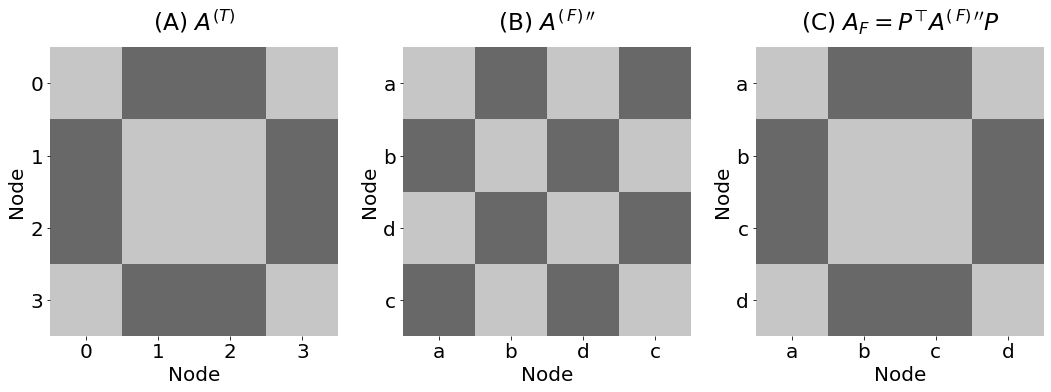
\includegraphics[width=\linewidth]{applications/ch8/Images/gm_fb_tw.png}
    \caption[Facebook and Twitter example, with permutations applied]{\textbf{(A)} The adjacency matrix for Twitter $A^{(T)}$, \textbf{(B)} The adjacency matrix for Facebook, $A^{(F)}''$, \textbf{(C)} The adjacency matrix for Facebook, after swapping nodes $c$ and $d$ via a permutation matrix.}
    \label{fig:ch8:gm:fb_tw}
\end{figure}

We want to construct a permutation matrix $P$, which will keep the nodes $a$ and $b$ in the same order, but swap nodes $c$ and $d$ in the node ordering. We can do this using the strategy that we developed above:

\begin{lstlisting}[style=python]
twitter = np.array([
    [0,1,1,0],
    [1,0,0,1],
    [1,0,0,1],
    [0,1,1,0]
])

facebook = np.array([
    [0,1,0,1],
    [1,0,1,0],
    [0,1,0,1],
    [1,0,1,0]
])

P = np.array([
    [1,0,0,0],
    [0,1,0,0],
    [0,0,0,1],
    [0,0,1,0]
])

fb_permutation = P.T @ facebook @ P
\end{lstlisting}
The Facebook adjacency matrix (after reshuffling) is shown in \ref{fig:ch8:gm:fb_tw}(C). Note that the permutation matrix swaps nodes $c$ and $d$, to recover the original node correspondence between Twitter and Facebook, and the networks are identical after pre- and post-multiplying by the permutation matrix.

\subsubsection*{Formalizing the Graph Matching Problem}

We will use this intuition to formulate the graph matching problem. For any two adjacency matrices $A, B$, we seek to minimize the cost function $g_P(A,B) = \left|| A - P^\top BP\right\|_F^2$ with the restriction that $P$ is a permuation matrix. This means that you want to figure out a way in which you can shuffle the rows and columns of $B$, such that it is as close as possible to $A$.
\subsubsection*{Generating a random permutation matrix}

Let's make ourselves a function which creates permutation matrices. Remember that for a permutation matrix, the entry $p_{ji}$ corresponds to a swap of rows/columns $i$ and $j$, depending on whether it is a row or column permutation (or being used for both).

\begin{lstlisting}[style=python]
def make_permutation(n):
    """
    A function that generates a permutation for n elements.
    
    1. Generate indices from 0 to n-1
    2. shuffle those indices
    3. Place 1s in the matrix P at the positions defined by the shuffled indices.
    """
    
    starting_indices = np.arange(n)
    destination_indices = np.random.permutation(n)
    P = np.zeros(shape=(n,n))
    P[destination_indices, starting_indices] = 1
    return P
\end{lstlisting}

\subsection{Finding a good permutation with gradient descent optimization}

To solve the optimization problem we described above, we'll use a variation of gradient descent. A gradient can be thought of as a vector valued slope; it is simply the slope of a function in all of its dimensions, at a single point in space. Gradient Descent is a common optimization method used to find minimums of functions.

\begin{figure}[h]
    \centering
    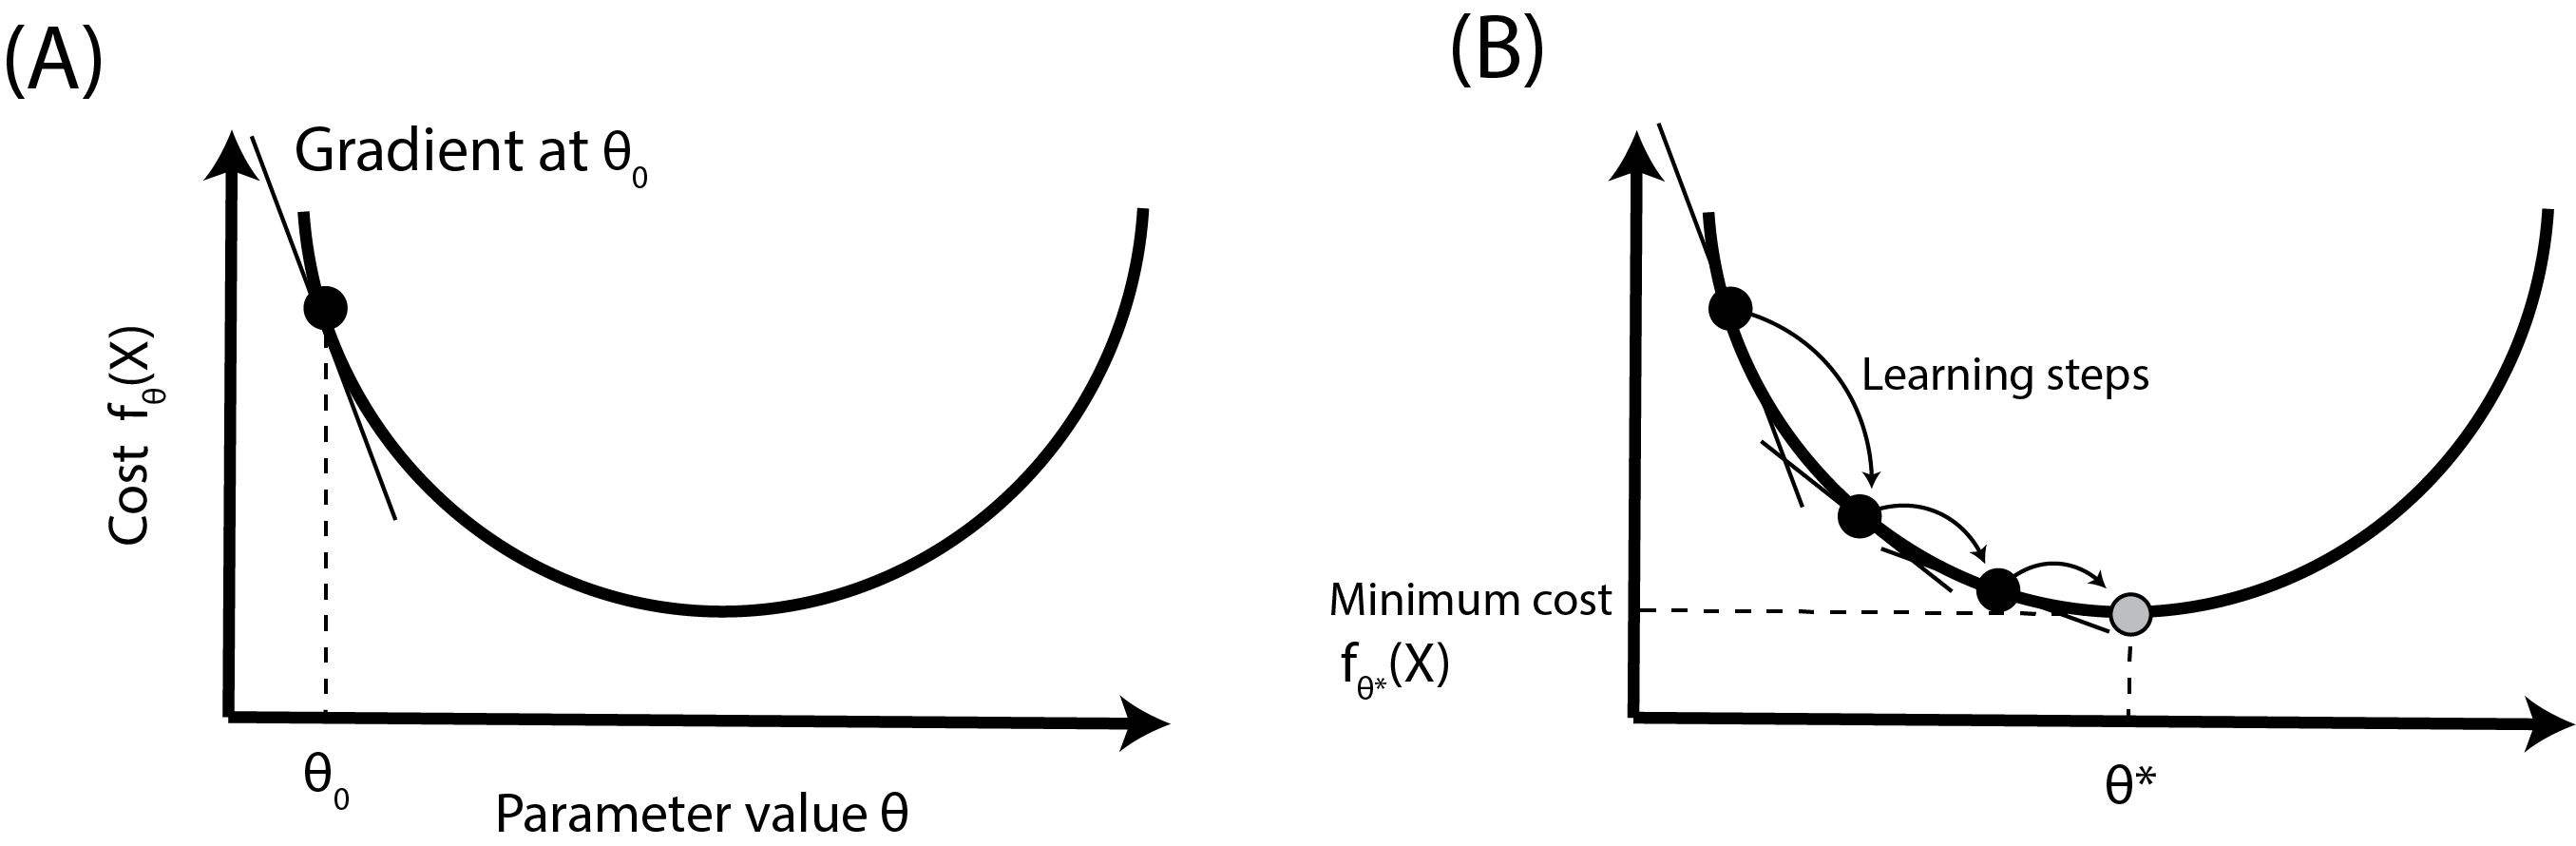
\includegraphics[width=\linewidth]{applications/ch8/Images/grad_desc.png}
    \caption[Gradient descent]{\textbf{(A)} the cost function with an initial starting position, \textbf{(B)} the cost function, optimized via gradient descent.}
    \label{fig:ch8:gm:grad_desc}
\end{figure}

The graph matching optimization problem, unfortunately, requires a background in nonlinear optimization, which is beyond the scope of this textbook. For that reason, we will focus heavily on the types of problems graph matching can solve in this chapter. If you do have such a background, please see the references for a more algorithmic understanding. For now, you can just think of the problem as being solved with something similar to gradient descent.

\begin{floatingbox}[h]\caption{Gradient Descent}

You can think of gradient descent like gravity. Consider an inspector using a golf ball to find the lowest point when installing a drain. The ball rolls down hill until it comes to a stop; once it stops, we know we've found the lowest point. Gradient descent works in a similar way, taking steps in the direction of the local gradient with respect to some parameter. Once the gradient is zero, a local minimum has been found and the algorithm is stopped. 

This process is illustrated in Figure \ref{fig:ch8:gm:grad_desc}, for a one-dimensional parameter $\theta$. The $y$-axis represents the cost $f_\theta(X)$ of a particular parameter choice $\theta$, given the data $X$ (solid line). In Figure \ref{fig:ch8:gm:grad_desc}(A), an initial parameter value $\theta_0$ is chosen to begin the optimization routine. The gradient is computed at the point $\theta_0$, which with a one-dimensional parameter, is the slope of the tangent line to $f_\theta(X)$ at $\theta_0$. Since the slope is negative, this indicates that increasing the value of the parameter an arbitrarily small amount past $\theta_0$ will decrease the cost. If the slope were positive, decreasing the value of the parameter an arbitrarily small amount past $\theta_0$ would decrease the cost. Figure \ref{fig:ch8:gm:grad_desc}(B) illustrates the effects of repeating this process. Successive ``learning steps'' repeat this process until the tangent line has a slope of zero, at which point a local minimum for the cost function $f_\theta(X)$ at $\theta^*$ has been found. 

The main steps of a gradient descent method are choosing a suitable initial position (can be chosen randomly), then gradually improving the cost function one step at a time, until the function is changing by a very small amount, converging to a minimum. The main issue with gradient descent is that it does not guarantee that you will find a global minimum, only that you will find a local minimum to your initial position (as long as your function is sufficiently smooth).  A commonly used strategy, and the one that we employ for graph matching, is known as the Fast Approximate Quadratic (FAQ) algorithm \cite{Vogelstein2015Apr}.

\end{floatingbox}

\subsection{Solving the graph matching problem}

For the example below, we will match two networks with a known node mapping that preserves a common network structure. To do this, we simulate a single sample from a $ER_8(0.5)$ random network. Then, we generate $B$ by randomly permuting the node labels of $A$. 

\begin{lstlisting}[style=python]
from graspologic.simulations import er_np

n = 8
p = 0.5

np.random.seed(1234)
A = er_np(n=n, p=p)
# make a permutation matrix
P = make_permutation(n)
B = P.T @ A @ P
disagreements = np.linalg.norm(A - B)**2
\end{lstlisting}

The network sample is shown in Figure \ref{fig:ch8:gm:simp_ex}(A), and the network after a random shuffling of the nodes is shown in Figure \ref{fig:ch8:gm:simp_ex}(B). 

\begin{figure}
    \centering
    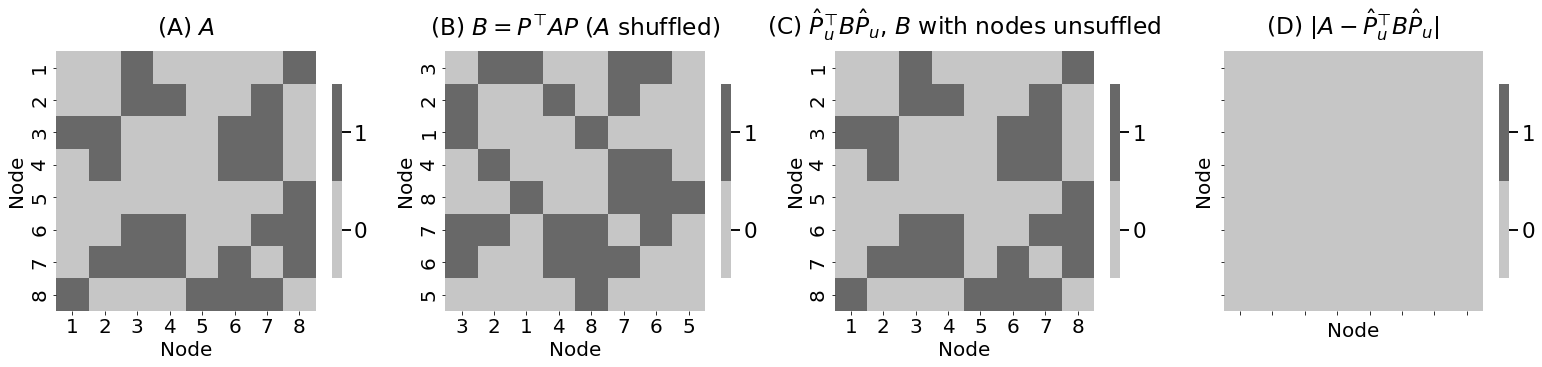
\includegraphics[width=\linewidth]{applications/ch8/Images/gm_simp_ex.png}
    \caption[Unshuffling to solve the graph matching problem]{\textbf{(A)} the original adjacency matrix, \textbf{(B)} the shuffled adjacency matrix $B$, using the random permutation $P$, \textbf{(C)} the unshuffling of $B$, after graph matching to $A$, \textbf{(D)} the edge disagreement matrix.}
    \label{fig:ch8:gm:simp_ex}
\end{figure}

Below, we create a model to solve the Graph Matching Problem using the \texttt{graph\_match} function. We pass in two networks, \texttt{A} and \texttt{B}, that we wish to ``match.''

\begin{lstlisting}[style=python]
from graspologic.match import graph_match

gmp = graph_match(A,B)
\end{lstlisting}

The \texttt{graph\_match} function returns a \texttt{MatchResult} object, which in its most straightforward application (the networks \texttt{A} and \texttt{B} have the same number of nodes), will return two indexing sets, \texttt{indices\_A} and \texttt{indices\_B}. Each element of these indexing sets correspond to the ``matches'' of nodes; that is, \texttt{indices\_A[j]} is ``matched'' to node \texttt{indices\_B}.

In this simple setting, \texttt{indices\_A} will just be the nodes ordered from $0$ to $n-1$, and indices \texttt{indices\_B} will be a map from the (current) indices of nodes in \texttt{B} that would align them to nodes in \texttt{A}.

We can use these indices to construct an ``unshuffling'' permutation matrix for network \texttt{B}, using the logic that we developed above for permutation matrices. We want a matrix $P_u = P^\top = P^{-1}$ where each element $p_{ij}$ is $1$ if $j = \texttt{indices\_B[i]}$, and $0$ otherwise. The original matrix, $P$, is the matrix that permuted $A$ to create $B$ in the first place.

\begin{lstlisting}[style=python]
def make_unshuffler(destination_indices):
    """
    A function which creates a permutation matrix P from a given permutation of the nodes.
    """
    n = len(destination_indices)
    P_u = np.zeros((n, n))
    starting_indices = np.arange(n)
    P_u[destination_indices, starting_indices] = 1
    return P_u

P_u = make_unshuffler(gmp.indices_B)
B_unshuffled = P_u.T @ B @ P_u
disagreements = np.linalg.norm(A - B_unshuffled)**2
\end{lstlisting}

In this case, we are estimating the unshuffling  matrix, so we produced an estimate $\hat P_u$. When we unshuffle $B$ with $\hat P_u$, we obtain the matrix $\hat P_u^\top B \hat P_u$, which is shown in Figure \ref{fig:ch8:gm:simp_ex}(C). Note that there are no edge disagreements between $\hat P^\top B \hat P$ and $A$, shown in Figure \ref{fig:ch8:gm:simp_ex}(D). 

The algorithm used is randomly initialized, so when you run this algorithm on your computer, you might not get a perfect unshuffling (but they should generally be pretty similar to what we got). 

\subsubsection*{The match ratio of nodes}

We can evaluate the quality of an unshuffling using the ratio of nodes which are correctly matched, called the \textit{match ratio}. We will use our knowledge of how $P$ behaves from Concept \ref{box:ch8:gm:unshuffle} to calculate this metric.

Because permutation matrices are orthogonal, $PP^\top = PP^{-1}$ is the identity matrix $I$. The match ratio is just the extent to which $P_u$ is the inverse of $P$, which is equivalent to the extent to which $P_u P$ is the identity matrix.

More specifically, every node which is incorrectly matched will correspond to an entry of $0$ along the diagonal of $PP_u$ (or equivalently, of $P_u P$).

With this in mind, we can just take the match ratio to be the fraction of times the diagonal of $P_uP$ of $PP_u$ is $1$:
\begin{align*}
    \text{match ratio}(P, P_u) = \frac{1}{n} \sum_{i = 1}^n \mathds 1\left\{(PP_u)_{ii} = 1\right\}
\end{align*}
where $P$ is a permutation matrix and $P_u$ is a proposed unshuffling matrix. The fancy looking function $\mathds 1\{x\}$ is just an indicator that has a value of $1$ if the statement inside the inside the curly braces is true, and $0$ if the statement inside the curly braces is false. So, here, it just has a value of $1$ if $(PP_u^\top)_{ii} = 1$, and a value of $0$ if $(PP_u^\top)_{ii} \neq 1$. We write a simple utility to do this, and then can call it on our permutation and un-shuffling matrix to see that the match ratio is $1$ here (we perfectly unshuffled $B$):

\begin{lstlisting}[style=python]
def match_ratio(P, Pu):
    n = len(P) # the number of nodes
    diag = np.diag(P @ Pu)
    return (diag == 1).sum() / n

print("match ratio: {:.3f}".format(match_ratio(P, P_unshuffle)))
# match ratio: 1.000
\end{lstlisting}

\subsection{Seeded graph matching (SGM) on correlated network pairs}

As networks become larger, they quickly become more difficult to match. One method to mitigate this difficulty is to use \textit{seeds}. \textit{Seeds} are a subset of matches that we already know before we perform the graph matching. For example, if we are given two networks $T$ and $F$ with 300 nodes each, we might already know ten node matches between $T$ and $F$. Having this prior information dramatically improves our ability to match the networks. 

To demonstrate the effectiveness of Seeded Graph Matching (\texttt{SGM}) \cite{Fishkind2019Mar, Lyzinski2014Jan}, the algorithm will be applied on a pair of simpler correlated SBM networks, which is an adaptation of the $\rho$-correlated $RDPG$ which we learned about in Section \ref{sec:ch5:multi:corr}. Like the $\rho$-correlated $RDPG$, the idea here is that we have two normal SBMs, but for any edge in the two networks $\mathbf a_{ij}$ and $\mathbf b_{ij}$, they will be correlated with correlation $\rho$. If there is sufficient correlation in edge structure between these two networks, we can hope to align the nodes of the two networks on the basis of this edge structure. The block matrix is:
\begin{align*}
B &= \begin{bmatrix} 
0.7 & 0.3 & 0.4\\
0.3 & 0.7 & 0.3\\
0.4 & 0.3 & 0.7
\end{bmatrix}
\end{align*}
The first $75$ nodes in the network will be from community one, the second $75$ nodes in the network will be from community two, and the third $75$ nodes in the network will be from community three:

\begin{lstlisting}[style=python]
from graspologic.simulations import sbm_corr

n_per_block = 75
n_blocks = 3
block_members = np.array(n_blocks * [n_per_block])
n_nodes = block_members.sum()
rho = 0.9
block_probs = np.array(
    [[0.7, 0.1, 0.4], 
     [0.1, 0.3, 0.1], 
     [0.4, 0.1, 0.7]]
)

A, B = sbm_corr(block_members, block_probs, rho)
disagreements = np.linalg.norm(A - B)**2
\end{lstlisting}

The networks $A$ and $B$ are shown in Figure \ref{fig:ch8:gm:sgm:ex_nets}(A) and (B). Note that the networks have a similar topological structure. 
\begin{figure}[h]
    \centering
    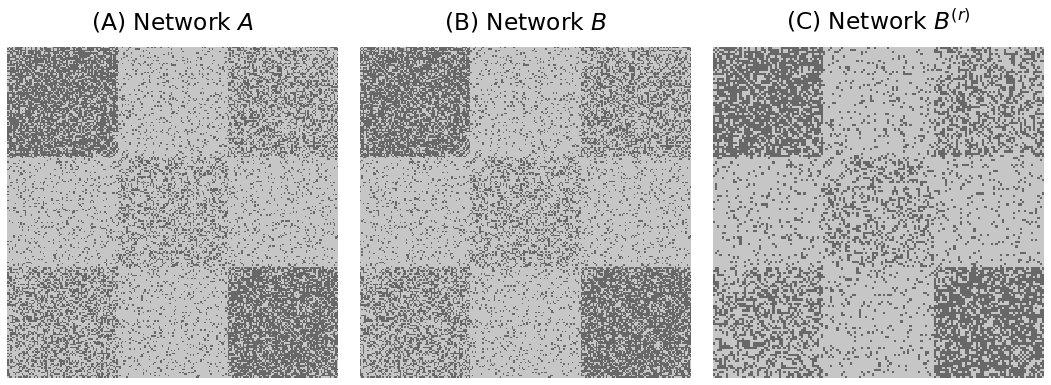
\includegraphics[width=\linewidth]{applications/ch8/Images/gm_sgm_nets.png}
    \caption[Seeded graph matching, networks (unshuffled)]{\textbf{(A)} The network $A$, \textbf{(B)} the network $B$ which is $\rho$-correlated to $A$, \textbf{(C)} the network $B^{(r)}$, which is the network $B$ with $35$ nodes removed per community.}
    \label{fig:ch8:gm:sgm:ex_nets}
\end{figure}

To emphasize the effectiveness of \texttt{SGM}, as well as why having seeds is important, we will randomly shuffle the vertices of network $B$. 

\begin{lstlisting}[style=python]
P = make_permutation(n_nodes)
B_shuffle = P.T @ B @ P
disagreements_shuffled = np.linalg.norm(A - B_shuffle)**2
print("Number of adjacency disagreements: {:d}".format(int(disagreements_shuffled)))
\end{lstlisting}

We will call this version of $B$ after shuffling $B^{(s)}$. The network $A$ and the shuffled network $B^{(s)}$ are shown in Figure \ref{fig:ch8:gm:sgm:ex}, along with the edge disagreements.

\begin{figure}[h]
    \centering
    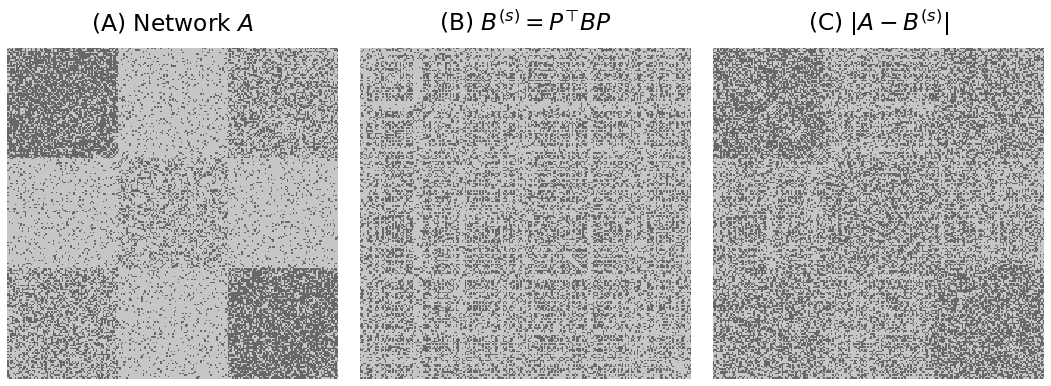
\includegraphics[width=\linewidth]{applications/ch8/Images/gm_seed_ex.png}
    \caption[Seeded graph matching example]{\textbf{(A)} the original network $A$, \textbf{(B)} the shuffled network $B^{(s)}$ which is $\rho$-correlated to $A$, \textbf{(C)} the edge disagreements between $A$ and $B^{(s)}$.}
    \label{fig:ch8:gm:sgm:ex}
\end{figure}

\paragraph*{Matching the networks without seeds}

First, we will run SGM on network $A$ and the shuffled network $B_s$ with no seeds, using a similar approach to the above


\begin{lstlisting}[style=python]
# fit with A and shuffled B
sgm = graph_match(A, B_shuffle)

# obtain unshuffled version of the shuffled B
P_unshuffle_noseed = make_unshuffler(sgm.indices_B)
B_unshuffle_noseed = P_unshuffle_noseed.T @ B_shuffle @ P_unshuffle_noseed

# compute the match ratio
n_verts = len(P)
match_ratio_noseed = np.count_nonzero(np.diag(P_unshuffle_noseed.T @ P))/n_verts
disagreements_noseed = np.linalg.norm(A - B_unshuffle_noseed)**2

print("Match Ratio, no seeds: {:.3f}".format(match_ratio_noseed))
print("Disagreements, no seeds: {:d}".format(int(disagreements_noseed)))
\end{lstlisting}

While the predicted unshuffling for $B$ was relatively successful in recovering the basic structure of the network $A$, we see that the number of edge disagreements between them is still quite high, and the match ratio of successfully unshuffled nodes is quite low (almost $0$). The original network $A$, the unshuffled network $\hat P_u^\top B^{(s)}\hat P_u$, and the edge disagreements between the original network and the unshuffled correlated network are shown in Figure \ref{fig:ch8:gm:sgm:noseed}. Note that the edge disagreements are fairly frequent.

\begin{figure}[h]
    \centering
    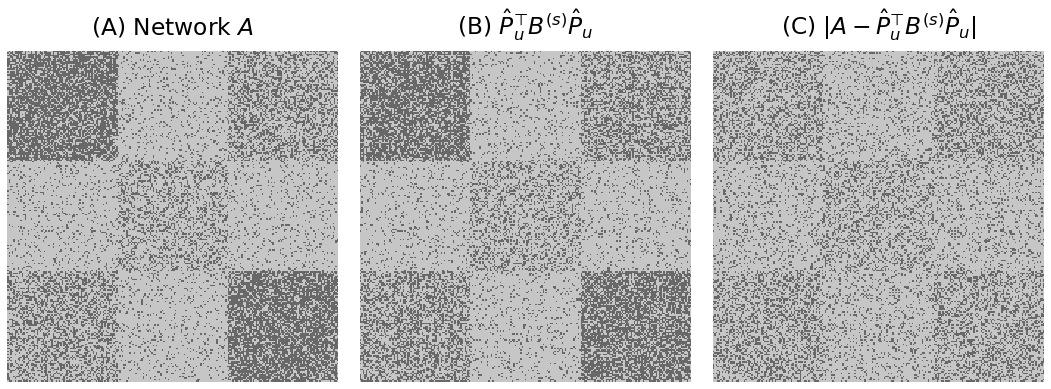
\includegraphics[width=\linewidth]{applications/ch8/Images/gm_sgm_noseed.png}
    \caption[Graph matching with no seeds]{\textbf{(A)} the original network $A$, \textbf{(B)} the unshuffling of the correlated network $\hat P_u^\top B^{(s)}\hat P_u$, \textbf{(C)} the edge disagreements between the original network and the unshuffled network.}
    \label{fig:ch8:gm:sgm:noseed}
\end{figure}

\paragraph*{Matching the networks with seeds}

Next, we will run SGM with 10 seeds randomly selected from the optimal permutation vector found ealier. Although 10 seeds is only about 3\% of the 300 node network, we will observe below how much more accurate the matching will be compared to having no seeds. We add a little helper function, which takes a permutation matrix and a desired number of seeds, and indicates where the identified seed nodes would be permuted to:

\begin{lstlisting}[style=python]
def gen_seeds(P, n_seeds):
    """
    A function to generate n_seeds seeds for a pair of matrices A and P^TBP
    which are initially matched, but P has been applied to permute the nodes
    of B.
    """
    n = P.shape[0]
    # obtain n_seeds random seeds from 1:n
    seeds = np.random.choice(n, size=n_seeds, replace=False)
    # use the permutation matrix to find where each seed was permuted to
    seeds_permuted = [np.where(P[i, :] == 1)[0] for i in seeds]
    return np.hstack(
        (seeds.reshape(n_seeds, 1), 
         np.array(seeds_permuted).reshape(n_seeds, 1))
    )
\end{lstlisting}

Next, we run seeded graph matching, using the \texttt{graph\_match} function from \texttt{graspologic}, by passing seeds as parameters:
\begin{lstlisting}[style=python]
nseeds = 10  # the number of seeds to use
# select ten nodes at random from A which will serve as seeds

# obtain seeds for nodes of A with nodes of B
seeds = gen_seeds(P, nseeds)

# run SGM with A and shuffled B, but provide the seed nodes from A as ref_seeds
# and the corresponding position of these seed nodes after shuffling as permuted_seeds
sgm = graph_match(A, B_shuffle, partial_match=seeds)
P_unshuffle_seeds = make_unshuffler(sgm.indices_B)

B_unshuffle_seeds = P_unshuffle_seeds.T @ B_shuffle @ P_unshuffle_seeds

match_ratio_seeds = match_ratio(P, P_unshuffle_seeds)
disagreements_seeds = np.linalg.norm(A - B_unshuffle_seeds)**2

print("Match Ratio, seeds: {:.3f}".format(match_ratio_seeds))
# Match Ratio with seeds: 1.000
print("Disagreements, seeds: {:d}".format(int(disagreements_seeds)))
\end{lstlisting}

The resulting unshuffling steps are shown in Figure \ref{fig:ch8:gm:sgm:seed}. Compared to Figure \ref{fig:ch8:gm:sgm:noseed}, we can see that the unshuffling produces far fewer edge disagreements than when we used unseeded graph matching. Further, using just $10$ seeds, the match ratio increased to at or near perfect (it should be near $1$). 

\begin{figure}[h]
    \centering
    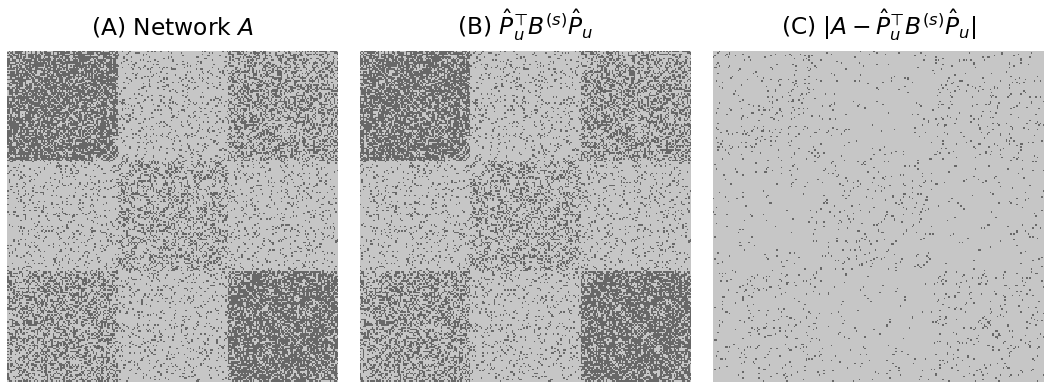
\includegraphics[width=\linewidth]{applications/ch8/Images/gm_sgm_seed.png}
    \caption[Seeded graph matching]{\textbf{(A)} the original matrix $A$, \textbf{(B)} the unshuffling of the correlated matrix $\hat P_u^\top B^{(s)}\hat P_u$ and \textbf{(C)} the edge disagreements when we graph match using seeds.}
    \label{fig:ch8:gm:sgm:seed}
\end{figure}

So, our conclusions can be summarized as follows:
\begin{enumerate}
    \item When one network is ``mis-aligned'' to another network, in that the nodes are not ordered the same but the network is otherwise identical, graph matching strategies can efficiently recover an unshuffling matrix to ``align'' the nodes between the two networks.
    \item When two networks have ``mis-aligned'' nodes and further are only correlated (rather than identical, up to the alignment of the nodes), graph matching strategies will, naively, struggle to find optimal solutions. However, if we can narrow down the scope of the problem via seeds, we can still yield precise solutions.
\end{enumerate}

\subsection{Padded graph matching}

From what we've seen so far, the two networks you are interested in matching nodes for must have the same number of nodes. In practice, this is a pretty restrictive limitation. You might come across pairs of networks where many, if not all, of the nodes in a smaller network are matched to a node in a larger network. In this case, you have a dilemma: how do you match the nodes between the networks, without knowing what to do with the extra nodes in the larger network?

We will do this through a technique called \textit{padded graph matching}, in which we add new nodes to the smaller network until it has the same number of nodes as the bigger network, and then we run graph matching on the resulting networks with an equal number of nodes.  We have two techniques to add these isolated nodes, naive and adaptive padding.

For these examples, we'll adjust our correlated network slightly. We'll keep our first network $A$ exactly like the network we sampled above from the $\rho$-SBM. For $B$, we'll arbitrarily take out the last 35 nodes of each block:

\begin{lstlisting}[style=python]
from graspologic.utils import remove_vertices
import numpy as np

nremove = 25

# nodes to remove from A
n_nodes_Brem = n_nodes - nremove*n_blocks
base_range = np.arange(n_per_block - nremove, n_per_block)
block_offsets = np.array([0, 75, 150])

# repeat a base range for each block and add block offsets
nodes_to_remove = np.repeat(base_range, len(block_offsets)) 
nodes_to_remove += np.tile(block_offsets, nremove)
nodes_to_retain = np.setdiff1d(np.arange(n_nodes), nodes_to_remove)

# use the remove_vertices function to remove nodes
B_rem = remove_vertices(B, nodes_to_remove)
\end{lstlisting}

In the above code, note the care taken to obtain node indices of the nodes from $B$ that are retained in $B^{(r)}$. This is so that we will be able to evaluate our graph matching after we apply graph matching techniques. The network with the last $35$ nodes removed from network $B$ is shown in Figure \ref{fig:ch8:gm:sgm:ex_nets}(C).

This leaves us with a network $B^{(r)}$ and corresponding underlying random network $\mathbf B^{(r)}$ in which there are only $150$ instead of $225$ nodes. These $150$ nodes are matched to $150$ of the $225$ nodes in $A$ and $\mathbf A$, respectively. We won't shuffle $B^{(r)}$ this time for visualization purposes, but the procedure below is identical when the network is shuffled.

Our task is to match the $150$ nodes in $B^{(r)}$ to their corresponding matched pair in $A$.

Behind the scenes, what we want to do is basically take the network $A$, and match $B^{(r)}$ to a subnetwork of $A$ induced by the nodes for which there is a corresponding matched pair. By this, what we mean is that we want to figure out which nodes in the larger network $A$ actually have a matched pair in $B^{(r)}$, and virtually ignore the other nodes entirely. In this case, the induced subnetwork of $A$ can be obtained like this:

\begin{lstlisting}[style=python]
A_induced = remove_vertices(A, nodes_to_remove)
\end{lstlisting}

which is exactly equivalent to:

\begin{lstlisting}[style=python]
A_induced = A[nodes_to_retain,:][:,nodes_to_retain]
\end{lstlisting}

\subsubsection*{Naive padded graph matching}

Through naive padding, we simply add isolated nodes to the smaller network (which is $B$, in your case), until the number of nodes in $B$ are equal to the number of nodes in $A$. If you remember from Section \ref{sec:ch4:regularization}, nodes in a simple network are just nodes which do not have any edges in the network) The padded version of $B$ can be obtained like this:

\begin{lstlisting}[style=python]
B_padded = np.pad(
    B_rem, 
    pad_width=[(0,nremove*n_blocks), (0, nremove*n_blocks)]
)
\end{lstlisting}

which makes the number of nodes in the two networks the same. The padded network is shown in Figure \ref{fig:ch8:gm:sgm:naive_padded}(B).

We can specify this by using the \texttt{graph\_match} function, using the argument \texttt{partial\_match=seeds}. Then, we re-run graph matching, optionally, using seeding, just like we did before. This time, after padding, the original seeds of the network should come from only the ``retained'' nodes; that is, we want to make sure our seeds actually come from the smaller network nodes that are actually part of network \texttt{B\_rem}, and are not the padded nodes that we added:

\begin{lstlisting}[style=python]
nseeds_padded = 5

# obtain which nodes of B will be the seeds to use, from the retained
# nodes in the network
rem_seeds = np.random.choice(n_nodes_Brem, 
              size=nseeds_padded, replace=False).reshape(-1, 1)

# obtain the nodes in A
ref_seeds = nodes_to_retain[rem_seeds.reshape(-1)].reshape(-1, 1)
seeds = np.hstack((ref_seeds, rem_seeds))

# run SGM with A and the padded network B
# since we didn't shuffle Br, the seeds are the same for both
gmp_naive = graph_match(A, B_padded, partial_match=seeds)

# unshuffle B using the padded version of B and the permutation identified
P_unshuffle = make_unshuffler(gmp_naive.indices_B)
B_unshuffle_seeds_naive = P_unshuffle.T @ B_padded @ P_unshuffle


\end{lstlisting}

The network after matching is shown in Figure \ref{fig:ch8:gm:sgm:naive_padded}(C). 

Unfortunately, The naive matching of $B^{(r)}$ after padding looks nothing like $A$ we were trying to match it to; particularly, notice that all of the ``padding nodes'' (with no edges) were simply ``matched'' with the second community of nodes. Notice that there is a large ``hole'' in the matched network in the middle, with very few edges. What happened?

\begin{figure}
    \centering
    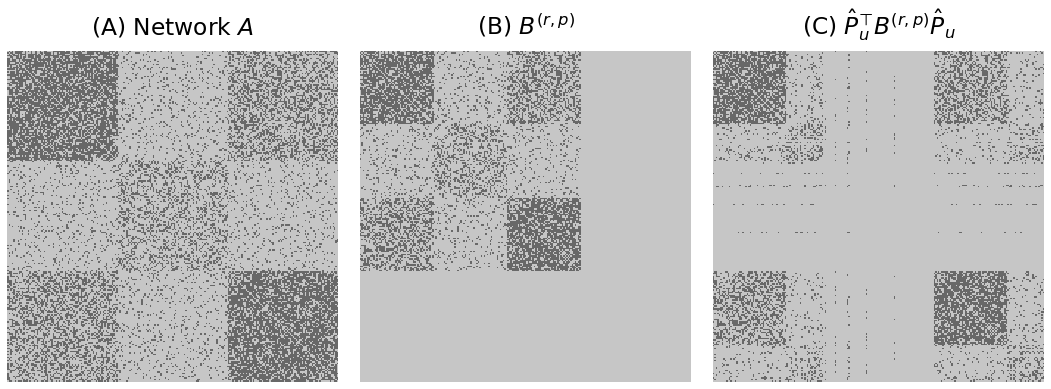
\includegraphics[width=\linewidth]{applications/ch8/Images/gm_naive.png}
    \caption[Naive padded graph matching]{\textbf{(A)} the original network $A$, \textbf{(B)}the network $B$ is $\rho$-correlated with $A$, has $35$ nodes removed to form $B^{(r)}$, and then has $35$ isolates added to pad $B^{(r,p)}$ to create the padded network, \textbf{(C)} the padded network after graph matching.}
    \label{fig:ch8:gm:sgm:naive_padded}
\end{figure}

\paragraph*{Naive matching matches padded nodes to low density subnetworks}

When we used this naive approach for padded graph matching, we made a critical error. We took the isolated nodes of $B$ that we added (just to make the number of nodes align) and attempted to, in some sense, consider these nodes as ``equals'' to the remaining nodes in the network in our matching. These nodes ended up being aligned to low-density subnetworks of $A$, which means that we allowed nodes that didn't really exist in $B^{(r)}$ (the padded nodes) to have a substantial role in the match quality. 

Looking at \ref{fig:ch8:gm:sgm:naive_padded}(C), let's consider the model that our networks were generated with. The average degree for nodes in community two are lower than the average degree for nodes in communities one and three, which means that these nodes will (in general) comprise the lowest density subnetwork of $A$. 

When we perform our matching, the isolated nodes from $B^{(r, p)}$ were ``aligned'' to the nodes in community two, which we can see in \ref{fig:ch8:gm:sgm:naive_padded}(C) by noting that the middle of the naive matched network is largely comprised of the nodes that we added synthetically with no edges (the isolates). Remember that these nodes are basically just placeholders, so we do not want them to have such a deciding role on our network.

To perform naive matching in \texttt{graspologic}, we can use the padding argument with the network \texttt{B\_rem} directly. This will match the nodes of the smaller of the two networks to the other, and the \texttt{indices\_*} return argument will indicate the nodes of each network that are matched to non-padding nodes:

\begin{lstlisting}[style=python]
# run naive padded SGM with A and the smaller network B_rem
# specifying padding="naive" internally does the same thing as we did above
gmp_naive = graph_match(A, B_rem, partial_match=seeds, padding="naive")

# unshuffle B using the network B with nodes removed
# and the permutation identified
P_unshuffle = make_unshuffler(gmp_naive.indices_B)
Brem_unshuffle_seeds_naive = P_unshuffle.T @ B_rem @ P_unshuffle
\end{lstlisting}

We can use \texttt{indices\_B} to evaluate the matching ratio and the number of agreements/disagreements, like we did before. If we recover the match perfectly, the unshuffling permutation matrix will be the identity matrix, since we did not reorder the nodes of $B^{(r)}$ when we formed the array \texttt{nodes\_to\_retain}:

\begin{lstlisting}[style=python]
# evaluate the match ratio by computing the permutation of the nodes of A,
# which should just be the identity matrix
match_ratio_naive = match_ratio(np.eye(len(nodes_to_retain)), P_unshuffle)
disagreements_naive = np.linalg.norm(A_induced - Brem_unshuffle_seeds_naive)**2
print("Match Ratio, naive padding: {:.3f}".format(match_ratio_naive))
# Match Ratio, naive padding: 0.333
print("Disagreements, naive padding: {:d}".format(int(disagreements_naive)))
\end{lstlisting}

Which gives us a low match ratio and a relatively high number of disagreements. As an exercise, plot \texttt{A\_induced}, and compare it to \texttt{B\_unshuffle\_seeds\_naive}. You should see that the networks look nothing alike, which means that our ``matching'' hasn't really done anything of value for us.

\subsubsection*{Adopted Padded Graph Matching}

Instead, what we want to do is match $B^{(r)}$ to the best fitting induced subnetwork of $A$. The key difference is that, in the ideal case, the subnetwork induced on $A$ is the set of nodes which were actually retained by $B$, and not just any ordinary subnetwork (or, in the case of naive padding, the lowest density subnetwork being matched to padding nodes).

To do this, we use a strategy called adopted padding, which is performed using `padding="adopted"` for the `GraphMatch` object. Through adopted padding, we normalize $A$ and $B^{(r)}$, to form $\tilde A$ and $\tilde B$, by multiplying the networks by 2, and then subtracting a matrix of $1$s. We again pad $\tilde B$ exactly like we did before, adding isolated nodes until the two networks have the same number of nodes. Through this normalization scheme, the padded nodes (which are not actual nodes in $B^{(r)}$) are \textit{downweighted}, such that they will tend to matter less in the cost function. What this has the effect of is making it so we will discount the padded nodes entirely when performing our graph matching, and will allow us to find the best induced subnetwork (on the nodes that are actually in the network $B^{(r)}$) instead. We perform this as follows:

\begin{lstlisting}[style=python]
Atilde = 2 * A - np.ones(A.shape[0])
Btilde = 2*B_rem - np.ones(B_rem.shape[0])
Btilde_padded = np.pad(Btilde, [(0,nremove*n_blocks), (0, nremove*n_blocks)])

# run SGM with Atilde and the padded network Btilde
# since we didn't shuffle Br, the seeds are the same for both
gmp_adopted = graph_match(Atilde, Btilde_padded, partial_match=seeds)

# unshuffle B using the padded version of B and the permutation identified
P_unshuffle = make_unshuffler(gmp_adopted.indices_B)
B_unshuffle_seeds_adopted = P_unshuffle.T @ B_padded @ P_unshuffle
\end{lstlisting}

The adopted padded and matched networks \texttt{A} and \texttt{B\_unshuffle\_seeds\_adopted} are shown in Figure \ref{fig:ch8:gm:sgm:adopted}(A) and Figure \ref{fig:ch8:gm:sgm:adopted}(B) respectively. Note that the isolated nodes tend to be dispersed to the last few nodes of each community, which is consistent with the nodes that were originally removed from the network. They are not restricted to the nodes in the lowest density induced subnetwork, as in Figure \ref{fig:ch8:gm:sgm:naive_padded}.

To evaluate this padding scheme, we can look evaluate the matching ratio and the on the subnetwork induced by the retained nodes. We can again do this by using \texttt{graspologic}, which will perform the above operation, and then induce the subnetwork of nodes retained by both networks (implied by the matching to non-padded nodes) automatically, like above:

\begin{lstlisting}[style=python]
# run SGM with A and Br with nodes removed
# since we didn't shuffle Br, the seeds are the same for both
gmp_adopted = graph_match(A, B_rem, partial_match=seeds, padding="adopted")

# unshuffle B using the padded version of B and the permutation identified
P_unshuffle = make_unshuffler(gmp_adopted.indices_B)
Brem_unshuffle_seeds_adopted = P_unshuffle.T @ B_rem @ P_unshuffle

match_ratio_adopted = match_ratio(np.eye(len(nodes_to_retain)), P_unshuffle)
disagreements_adopted = np.linalg.norm(A_induced - Brem_unshuffle_seeds_adopted)**2
print("Match Ratio, adopted padding: {:.3f}".format(match_ratio_adopted))
# Match Ratio, adopted padding: 1.000
print("Disagreements, adopted padding: {:d}".format(int(disagreements_adopted)))
\end{lstlisting}

Using adopted matching has increased the match ratio to perfect, and the number of disagreements has been dramatically reduced.

The network \texttt{A\_induced} induced by the nodes included is shown in Figure \ref{fig:ch8:gm:sgm:adopted}(C), alongside the network \texttt{Brem\_unshuffle\_seeds\_adopted} with adopted matching in Figure \ref{fig:ch8:gm:sgm:adopted}(D). This appears much more reasonable than the outcome we saw in Figure \ref{fig:ch8:gm:sgm:naive_padded}.

\begin{figure}
    \centering
    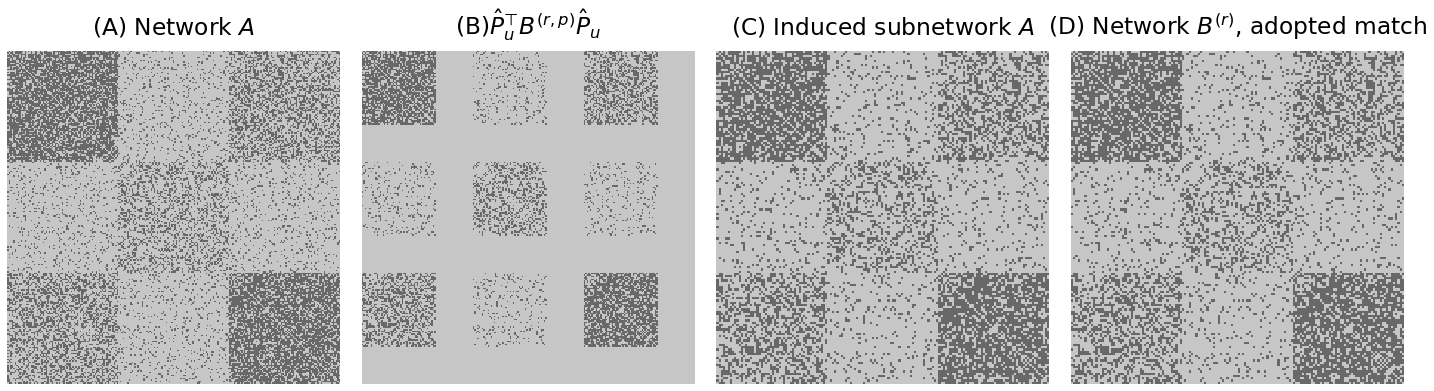
\includegraphics[width=\linewidth]{applications/ch8/Images/gm_adopted.png}
    \caption{\textbf{(A)} The network $A$, \textbf{(B)} the padded correlated network $B^{(r,p)}$ after row/column permutation by $\hat P_u$ via adopted matching, \textbf{(C)} the subnetwork of $A$ induced by the nodes in $B^{(r)}$, \textbf{(D)} the correlated network $B^{(r)}$ after row/column permutation by $\hat P_u$.}
    \label{fig:ch8:gm:sgm:adopted}
\end{figure}

\begin{floatingbox}[h]\caption{Remark: Vertex Nomination via Seeded Graph Matching}
It is often the case that we might have two networks $A^{(1)}$ and $A^{(2)}$, and we might want to ask which node or set of nodes in a second network are ``maximally similar'' to a given node (or set of nodes) of interest in the first network. Let's call this node $i^{(1)}$. This can be conceptualized as a form of the vertex nomination problem from Section \ref{sec:ch7:vn}, where we have a node of interest (or set of nodes of interest) and want to produce a \textit{nomination list} of possible nodes in the network $A^{(2)}$ that our node(s) of interest in the network $A^{(1)}$ are most similar to. 

Given that the solution to the graph matching problem is non-deterministic, in that running it twice might produce a slightly different matching (because we use stochastic gradient descent), we can estimate a nomination list by computing the number of times each node $j^{(2)}$ in network $2$ are matched to node $i^{(1)}$. Then, we can order the nomination list by the nodes that are most frequently matched to node $i^{(1)}$. This procedure is known as \texttt{VNviaSGM} \cite{Patsolic2020Jun}.
\end{floatingbox}

\newpage
